\documentclass[11pt, oneside]{article}   	% use "amsart" instead of "article" for AMSLaTeX format
\usepackage{geometry}                		% See geometry.pdf to learn the layout options. There are lots.
\geometry{letterpaper}                   		% ... or a4paper or a5paper or ... 
%\geometry{landscape}                		% Activate for for rotated page geometry
%\usepackage[parfill]{parskip}    		% Activate to begin paragraphs with an empty line rather than an indent
\usepackage{graphicx}				% Use pdf, png, jpg, or eps� with pdflatex; use eps in DVI mode
								% TeX will automatically convert eps --> pdf in pdflatex		
\usepackage{amssymb}
\usepackage{amsmath}

\title{Introduction to Taylor Series}
%\author{The Author}
\date{}							% Activate to display a given date or no date

\graphicspath{{/Users/telliott_admin/Dropbox/Tex/png/}}
\begin{document}

\maketitle
%\section{}
% \subsection*{R code}
% \begin{lstlisting}  \end{lstlisting}
% \begin{center} 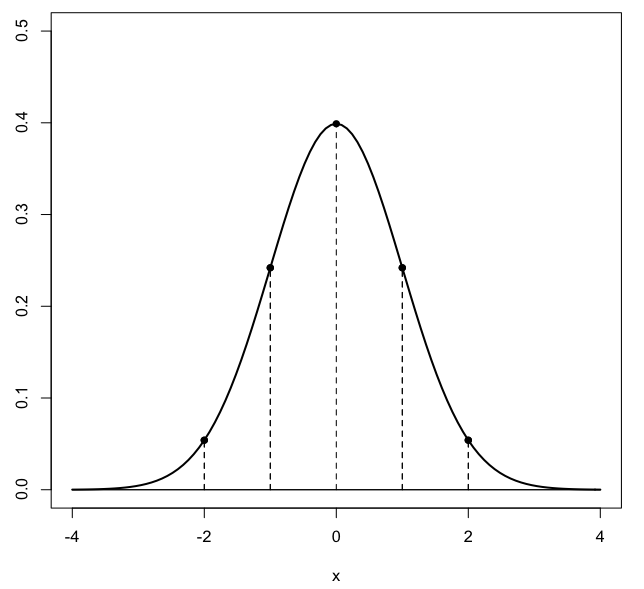
\includegraphics [scale=0.4] {gauss3.png} \end{center}
% \begin{bmatrix} a  &  b \\ c  &  d \end{bmatrix}
% \bigg |_

\large
\noindent In this short write-up I want to introduce the Taylor Series.  Rather than try to derive it, I will just write out the definition

\[ f(x) = f(a) + \frac{f'(a)}{1!}(x-a) + \frac{f''(a)}{2!}(x-a)^2 + \frac{f'''(a)}{3!}(x-a)^3 + \cdots \]
where $f'(a)$ is the first derivative of $f(x)$ evaluated at $a$, and so on.
This is a (possibly) infinite series and the nth term is 
\[ \frac{f^{(n)}(a)}{n!}(x-a)^n \]

This says that the Taylor series of the function $f(x)$ "near" a point $x=a$ is equal to this sum.

The beauty of Taylor Series (despite its complexity) is that it turns any differentiable function into a polynomial.  Polynomials are easy to integrate and work with.

The first thing to say about Taylor Series is they give the correct answer for functions that we know.  For example, suppose we have 
\[ f(x) = ax^2 + bx + c = 1 \]
We get the derivatives and evaluate them "near" the point $x=0$.
\[ f(x) = ax^2 + bx + c = c \]
\[ f'(x) = 2ax + b = b \]
\[ f''(x) = 2a \]
The series is then
\[ f(x) = c + b(x) + \frac{21}{2!}(x)^2 + \cdots \]
But there are no more terms.  That's it.  And this is just
\[ f(x) = c + bx + ax^2 \]

Let's take a second example.  Suppose $f(x) = e^x$ and again, we evaluate "near" $x=0$.  We have
\[ f(x) = e^x = 1 \]
\[ f'(x) = e^x = 1 \]
\[ f''(x) = e^x = 1 \]
The series is
\[ f(x) = e^x = f(0) + \frac{f'(0)}{1!}(x-0) + \frac{f''(0)}{2!}(x-0)^2 + \frac{f'''(0)}{3!}(x-0)^3 + \cdots \]
\[ f(x) = 1 + \frac{1}{1!}x + \frac{1}{2!}x^2 + \frac{1}{3!}x^3 + \cdots \]
\[ f(x) = 1 + x + \frac{x^2}{2!} + \frac{x^3}{3!} + \cdots \]
Which matches what we already know about $e^x$.  For example, it is obvious that 
\[ \frac{d}{dx}e^x = e^x \]

Let's try to find something new.  Suppose we expand $f(x) = cos\ x$ near $x=0$
\[ f(x) = cos \ x = cos \ 0 = 1 \]
\[ f'(x) = -sin \ x = -sin \ 0 = 0 \]
\[ f''(x) =  -cos \ x -cos \ 0 = -1 \]
\[ f'''(x) =  sin \ x = sin \ 0 = 0 \]
\[ f''''(x) =  cos \ x =  cos \ 0 = 1 \]
and this continues in a cycle with period 4.
The series is
\[ f(x) = f(a) + \frac{f'(a)}{1!}(x-a) + \frac{f''(a)}{2!}(x-a)^2 + \frac{f'''(a)}{3!}(x-a)^3 + \cdots \]
\[ f(x) = cos \ x = 1 - \frac{1}{2!}(x-0)^2 + \frac{1}{4!}(x-0)^4 + \cdots \]
\[ f(x) = cos \ x = 1 - \frac{x^2}{2!} + \frac{x^4}{4!} + \cdots \]

Similarly, for $f(x) = sin \ x$ near $x=0$
\[ f(x) = sin \ x = 0 \]
\[ f'(x) = cos \ x = 1 \]
\[ f''(x) = -sin \ x = 0 \]
\[ f'''(x) =  -cos \ x = -1 \]
\[ f''''(x) =  sin \ x = 0 \]
The series is
\[ f(x) = f(a) + \frac{f'(a)}{1!}(x-a) + \frac{f''(a)}{2!}(x-a)^2 + \frac{f'''(a)}{3!}(x-a)^3 + \cdots \]
\[ f(x) = sin \ x = x - \frac{1}{3!}(x-0)^3 + \frac{1}{5!}(x-0)^5 + \cdots \]
\[ f(x) = sin \ x = x - \frac{x^3}{3!} + \frac{x^5}{5!} + \cdots \]

Other examples..

\end{document}  